\subsection{Application Architecture}

\begin{figure}[hbt]
	\centering
	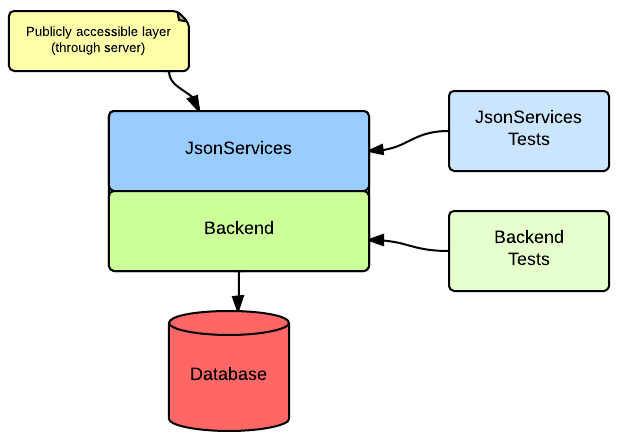
\includegraphics[scale=0.5]{./p1design/layers.png}
	\caption{The different layers in the application, showing how tests interact with
        the different layers, and how JsonServices builds on Backend and is the accessible
        layer.}
	\label{fig:layers}
\end{figure}

When designing the general architecture of the application, we decided on a simple, layered approach.
This was done to separate any business logic from actual presentational code. In the case of an online
API, the actual API is the presentational part (not to be confused with the client, which was developed
separately from the server).

The \verb+JsonService+ project uses the logic availible through \verb+Backend+ library. Each of these has
a testing library tied to it. The \verb+Backend+ utilizes a MSSQL database.